\section{Prototypes}
This section will describe the setup of the prototypes developed during this project.

\subsection{Prototype \#1}
The first prototype was an Android phone application that showed the location of the user, the direction the phone was pointing, and the devices that were being pointed at.
The application used a 10x10 grid to simulate a square room in which the user and the devices to be controlled were located.
A set of imaginary devices was hardcoded into the application with fixed positions and the grid would look like the one shown in table \ref{table/prototype-grid}.
The user is positioned in the center at \{5,5\} by default. This position can be changed by using the \texttt{Up}, \texttt{Down}, \texttt{Left} and \texttt{Right} buttons.
When the user's direction changes a list of devices being pointed at is acquired by calculating the angle between the user's position and the position of each device.
A screenshot of this application is shown in figure \ref{fig:first-prototype-screenshot}.

\begin{table}[]
\centering
\begin{tabular}{|l|l|l|l|l|l|l|l|l|l|}
\hline
 &  &  &  &  &  &  &  &  & Stereo \\ \hline
 &  &  &  &  &  &  &  &  &  \\ \hline
 &  &  &  &  &  & \begin{tabular}[c]{@{}l@{}}Coffee\\ Maker\end{tabular} &  &  &  \\ \hline
 &  &  &  &  &  &  &  &  &  \\ \hline
\begin{tabular}[c]{@{}l@{}}Garage\\ Door\end{tabular} &  &  &  &  &  &  &  &  &  \\ \hline
 &  & Lamp 2 &  &  &  &  &  &  &  \\ \hline
 &  &  &  &  &  &  &  &  &  \\ \hline
 &  &  &  &  &  &  &  &  &  \\ \hline
 &  &  &  &  &  &  &  &  &  \\ \hline
Lamp 1 &  &  &  &  & TV &  &  &  &  \\ \hline
\end{tabular}
\caption{Grid showing the position of devices. Lamp 1 is located at \{0,0\} and Stereo is located at \{9,9\}}
\label{table/prototype-grid}
\end{table}

\begin{figure}[]
    \centering
    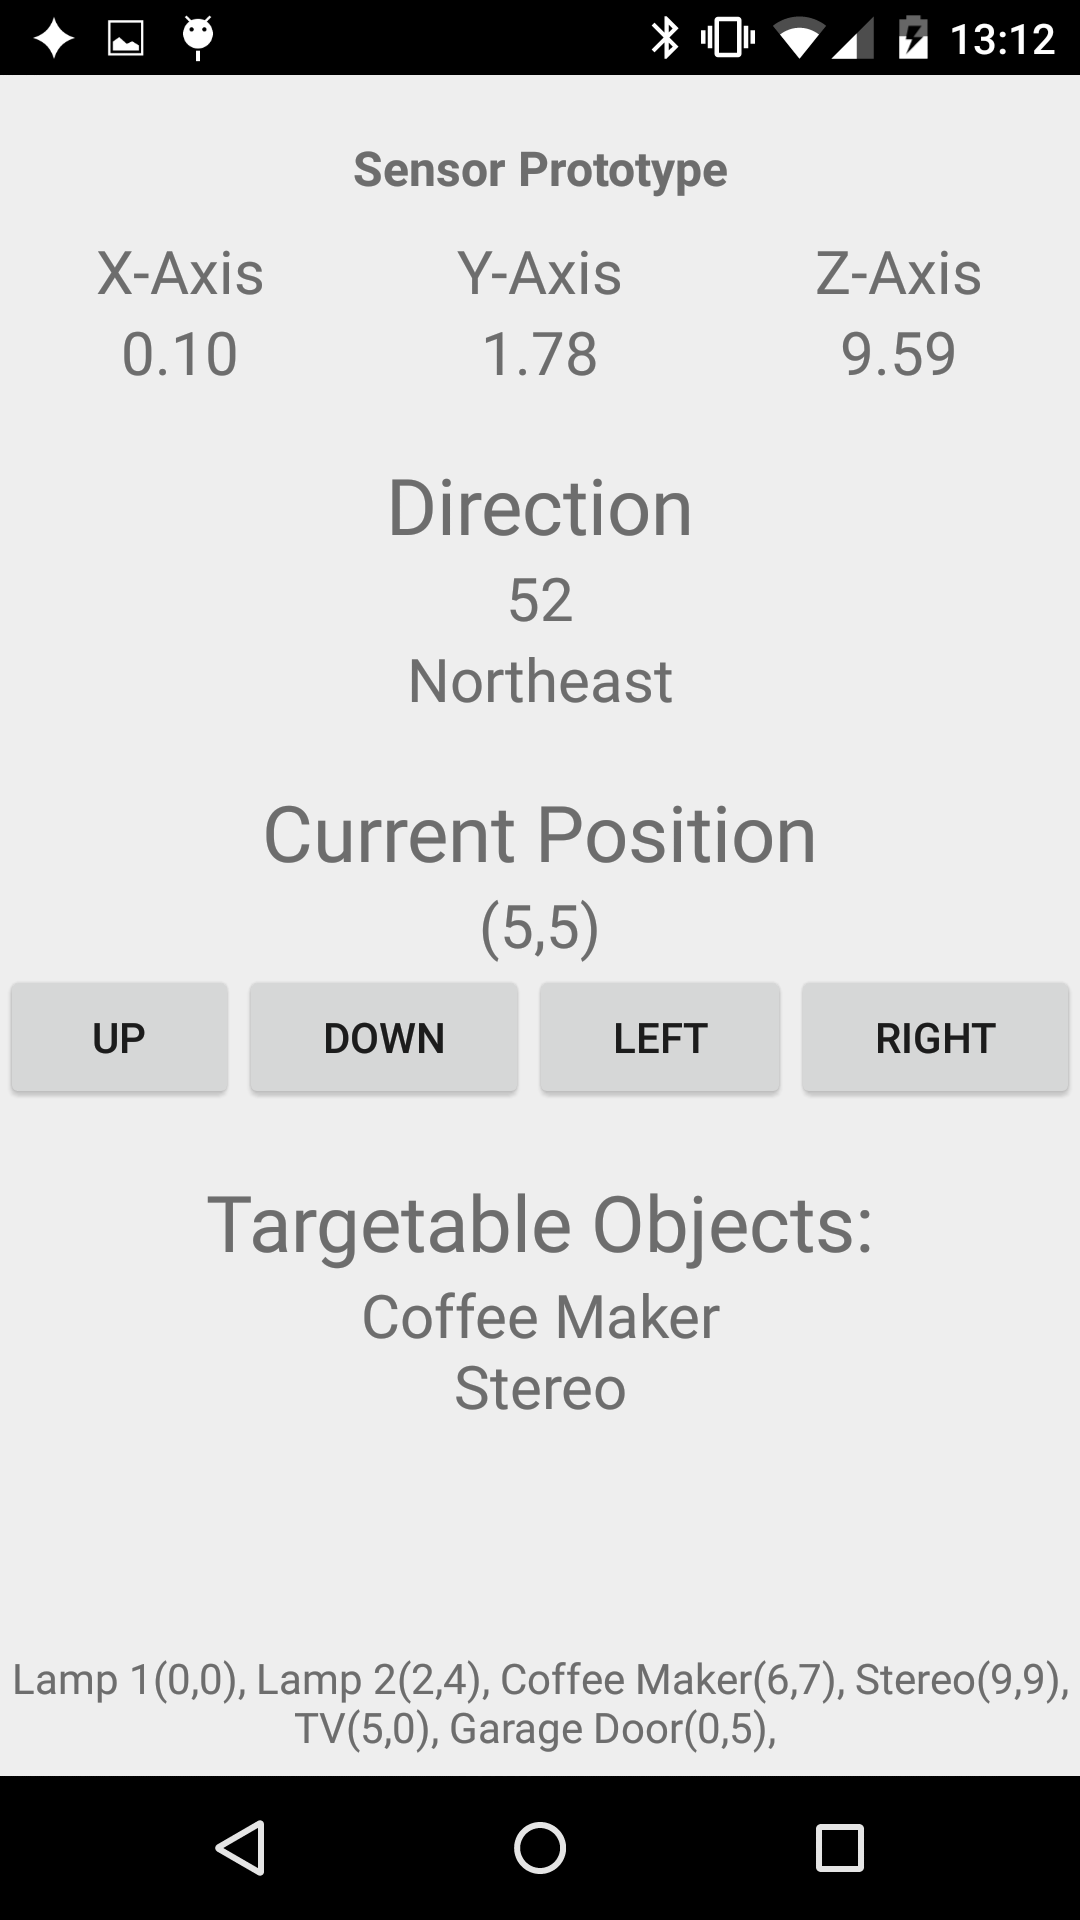
\includegraphics[scale=0.2]{images/Android_Prototype1_1.png}
    \caption{Screenshot of the first prototype.}
    \label{fig:first-prototype-screenshot}
\end{figure}